
\subsubsection{2012: Skillen et al.}
%\citep{skillen2012ontological}
\label{sec:skillen}

Within an application personalization within mobile 
environments~\citet{skillen2012ontological} present a User Profile Ontology 
which is able of modelling dynamic components. The ontology considers both 
static and dynamic aspects of the user mainly focused on his/her behaviour 
changes. The user capabilities are also taken into account for the user profile. 
Capabilities are defined as the extent to which the user has an ability (i.e., 
physical, emotional or cognitive) to carry out some activities. User's interests 
and several context parameters are also considered in the ontology to cover 
context-aware environments. Figure~\ref{fig:skillen_ontology} overviews the 
User Profile Ontology classes, object properties and data properties presented 
by~\citeauthor{skillen2012ontological}.

\begin{figure}
\centering
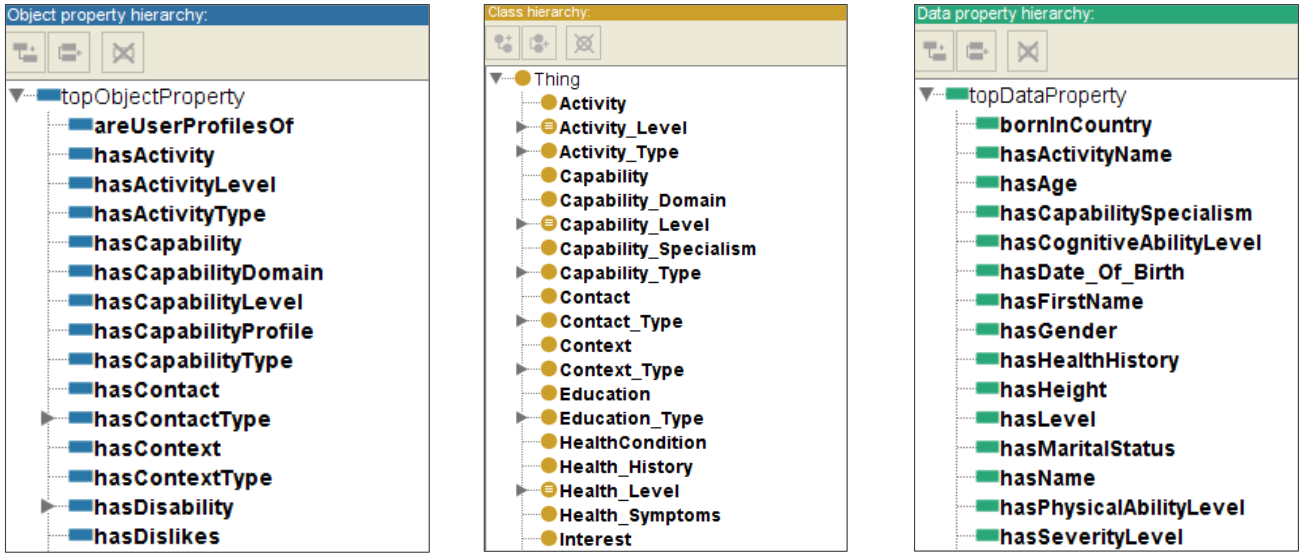
\includegraphics[width=0.70\textwidth]{skillen_ontology.png}
\caption{An overview of the User Profile Ontology classes, object properties and 
data properties~\citep{skillen2012ontological}.}
\label{fig:skillen_ontology}
\end{figure}